\documentclass[12pt]{article}

%\renewcommand{\baselinestretch}{1.65}
\usepackage{amsmath,graphicx,bbm,amssymb}
\usepackage{txfonts}
\usepackage{array}
\usepackage{subfigure}
\usepackage{caption}
\usepackage{color}
\usepackage{tikz}
\usetikzlibrary{arrows} 
\usetikzlibrary{shapes.multipart}
\usetikzlibrary{shapes.misc, positioning}
\usepackage{float}
\usepackage{calc}
\usepackage{multirow}
\usepackage{fancyhdr}
\usepackage{colortbl}
\usepackage[colorlinks=true,linkcolor=blue,citecolor=blue,urlcolor=blue]{hyperref}
\usepackage[hmargin=1.5cm, top=2.5cm, bottom=2.5cm]{geometry}

\newcommand{\procspie}{Proc. SPIE } 
\newcommand{\pasp}{Publications of the Astronomical Society of the Pacific } 
\newcommand{\aap}{Astron. \& Astrophys. } 
\newcommand{\mnras}{M.N.R.A.S } 

\newcommand{\module}[1]{\left\vert #1 \right\vert}
\newcommand{\norme}[1]{\left\vert\left\vert #1 \right\vert\right\vert}
\newcommand{\para}[1]{\left(#1\right)}
\newcommand{\cro}[1]{\left[#1\right]}
\newcommand{\aver}[1]{\left\langle #1 \right\rangle}
\newcommand{\bra}[1]{\left\lbrace #1 \right\rbrace}
\newcommand{\xth}[1]{#1^{\text{th}}}
\newcommand{\otfdl}{\text{OTF}_\text{DL}}

\newcommand{\rz}{r_0}
\newcommand{\lz}{L_0}
\newcommand{\cnh}{C_n^2(h)}
\newcommand{\cnhl}{C_n^2(h_l)}
\newcommand{\nwfs}{\text{n}_\text{wfs}}
\newcommand{\R}{\boldsymbol{\text{R}}}
\newcommand{\Mc}{\boldsymbol{\text{M}_c}}
\newcommand{\thSrc}{\boldsymbol{\theta}_\text{src}}
\newcommand{\thGs}{\boldsymbol{\theta}_\text{gs}}
\newcommand{\thNgs}{\boldsymbol{\theta}_\text{ngs}}
\newcommand{\thLgs}{\boldsymbol{\theta}_\text{lgs}}
\newcommand{\rbb}{\boldsymbol{r}}
\newcommand{\rbun}{\boldsymbol{r}_1}
\newcommand{\rbdeux}{\boldsymbol{r}_2}
\newcommand{\rhob}{\boldsymbol{\rho}}
\newcommand{\ubl}{\boldsymbol{u}/\lambda}
\newcommand{\ub}{\boldsymbol{u}}
\newcommand{\alphab}{\boldsymbol{\alpha}}
\newcommand{\TTout}{\boldsymbol{\text{TT}}_\text{out}}
\newcommand{\TTonly}{\boldsymbol{\text{TT}}_\text{only}}
\newcommand{\otf}[1]{\text{OTF}_{#1}}
\newcommand{\atf}[1]{\text{ATF}_{#1}}
\newcommand{\cov}[1]{\mathcal{C}_{#1}}
\newcommand{\eps}{\boldsymbol{\varepsilon}}
\newcommand{\epspara}{\boldsymbol{\varepsilon}_\parallel}
\newcommand{\hi}{\boldsymbol{h}_i}
\newcommand{\hj}{\boldsymbol{h}_j}

\title{KASP Technical notes \#09:\\ Focal plane profiler with KASP: concept and results on the HeNOS bench.}
\author{O. Beltramo-Martin\footnote{olivier.martin@lam.fr}, C.~M. Correia}
\date{}

% Option to view page numbers
%\pagestyle{plain} % change to \pagestyle{plain} for page numbers   
\setcounter{page}{1}
\fancyhead[LO,LE]{KASP Technical notes \#09}
\fancyhead[RE,RO]{O. Beltramo-Martin}
\pagestyle{fancy} 
\setlength{\parindent}{0cm}

\begin{document}


\maketitle
\rule{\columnwidth}{0.1mm}
\tableofcontents
\rule{\columnwidth}{0.1mm}
\section{Purpose}

We describe the Focal Plane Profiler~(FPP) concept, as a model-fitting algorithm handling $\cnh$ values to minimize residual on PSF reconstruction. We detail the principle of the method of results obtained on HeNOS bench data.

\section{The FPP concept}
\subsection{Motivations}

PSF reconstruction involves two capabilities: the first one requires to handle AO telemetry to reconstruct the PSF on-axis, while the second one consists in extrapolating the PSF anywhere across the field. This latest step is based on the atmospheric turbulence description as the seeing value, $\cnh$ and outer scale profiles. The common approach takes these information as priors, either provided by an external profiler (MASS/DIMM, SLODAR or SCIDAR for instance) or estimated through AO telemetry for multiple-WFS based AO systems.\\

PSF-R must achieve a proper PSF reconstruction for science data processing purpose. In particular we aim at improving astrophysics estimates, such photometry and astrometry, by providing a better estimation of what the PSF is really is, compared to focal-plane methods, that could suffer by sources overlapping and confusion noise. 

However focal plane images contain the information that really matters for, i.e. the PSF. There's no point in performing PSF-R is the output product is far from what we observe at the science instrument focal plane.\\

Here comes the idea of gathering AO telemetry and focal-plane images to produce the best estimation of the PSF. Basically, we propose a \emph{Learn \& Apply} fashion for improving the reconstruction based on three steps~:
\begin{itemize}
	\item[$\bullet$] Produce a reconstruction of the on-axis PSF from $\cnh$ non-scaled terms, i.e. telemetry and NCPA residual.
	\item[$\bullet$] Define a PSF model as the convolution of the on-axis PSF with a $\cnh$-dependent filter, including anisoplanatism (angular, focal and tip-tilt), fitting error~(PSF wings) and aliasing error. The two latest terms are only $\rz$-dependent. Then we least-square minimize the residual produced by the observations/model difference in fitting the $\cnh$ profile.
	\item[$\bullet$] We derive the closest version of the model we have in injecting retrieved fitted parameters from the previous step.
\end{itemize}

Several points can be discussed for optimizing this procedure. The way the problem is posed needs to be inverted and requires specific method. For the sake of simplicity of make sure the concept is feasible, we've opted for a model-fitting procedure but alternative option exists. In particular it may be possible to derive the cost function gradient with respect to the $\cnh$ profile.\\ 

In any case this problem need to be regularized to achieve a proper estimation. The way is done in the actual version of the FPP is to concatenate several measured PSF into a single array. For PSF discretized on $N\times N$ samples, we finally dispose of a meta array sizing $N\times (N\times n_\text{src})$ with $n_\text{src}$ the number of picked-off PSFs from the focal plane image. In particular, NCPA residual may cause PSF core elongation that could confuse the model-fitting procedure. Handling several PSF across the field is a way to mitigate this problem. Also, including the on-axis PSF, what is only seeing-dependent, observed through the focal-image would make the seeing estimation more robust.


\subsection{PSF model}


The PSF model we're working with is the usual one based on Optical transfer function~(OTF) multiplication as:
\begin{equation}\label{E:model}
	\otf{\Delta}(\ubl,\cnh) = \otf{0}(\ubl) \times \otf{\perp}(\ubl,\rz) \times \otf{\text{Alias}}(\ubl,\rz) \times \atf{\Delta}(\ubl,\cnh),
\end{equation}
where the Freid's parameter $\rz$ is derived from the integral of $\cnh$ along altitude~:
\begin{equation}
	\rz = \para{0.423\times\para{\dfrac{2\pi}{\lambda}}^2\times\dfrac{1}{\cos{(\gamma)}}\times\int_{\mathcal{R}} \cnhl dh}^{-3/5},
\end{equation}
with $\gamma$ the zenithal angle. See the KASP note \#03 more description. Our point is to get a fast-computational model depending on the $\cnh$ values. We detail each model component herein. 

If assuming altitude layers are known, or discretized at a desired sampling along altitude , we get as many parameters as number of layer we consider to get the $\cnh$ profile. Also, we may include the outer scale profile, or at least an integrated value kept constant for each altitude. In the following we've considered the outer scale as infinite on Henos, meaning we assume outer scale effect are not impacting PSF. For further deployment of this method on NIRC2 wide-field observations, outer scale must be considered. The FPP algorithm embedded into KASP offers the possibility to fit an outer scale profile or integrated value and layers heights as well.

\subsubsection{Fitting model}
We base the computation of this term on a Fourier approach, consisting in modeling the perpendicular phase PSD as the atmosphere Von-K\'arm\`an PSD released from low spatial frequencies lower than $k_c$ the DM-cut off frequency~:
\begin{equation}
\otf{\perp} = \exp(\mathcal{C}_{\perp}(\rhob) - \mathcal{C}_{\perp}(0) ),
\end{equation}
where $	\mathcal{C}_{\perp}(\rhob)$ is the covariance map derived by the phase PSD using the Wiener-Khintchine theorem~:
\begin{equation}
\mathcal{C}_{\perp}(\rhob) = \mathcal{F}\cro{\tilde{\Phi}_\text{atm}(\boldsymbol{k})\times {\Pi}_{k_c} },
\end{equation}
with ${\Pi}_{k_c}$ the gate function in the frequency domain~:
\begin{equation}
{\Pi}_{k_c}(\boldsymbol{k}) = \left\lbrace 
\begin{aligned}
& 0\quad \text{if}\quad k_x \leq k_c \: | \: k_y \leq k_c\\
& 1\quad \text{else}
\end{aligned}
\right.
\end{equation}

\subsubsection{Aliasing model}
Aliasing error comes from the aliased phase that creates a signal and that is reconstructed onto the DM commands and affects the in-band correcting part of the AO PSF. We follow the same procedure as for the fitting error~:
\begin{equation}
\otf{\text{Alias}} = \exp(\mathcal{C}_{\text{Alias}}(\rhob) - \mathcal{C}_{\text{Alias}}(0) ),
\end{equation}
where the covariance map id derived from~:
\begin{equation} \label{E:covalias}
\mathcal{C}_{\text{Alias}}(\rhob) = \mathcal{F}\cro{\tilde{\Phi}_\text{Alias}(\boldsymbol{k})}
\end{equation}
The aliased phase results from the spatial sampling of the phase every $1/2d$. The aliasing PSD is thus a sum of the initial spectrum shifted by an integer time $1/d$. The calculation includes the filtering through the WFS reconstructor $\tilde{\R}$ and the AO system temporal transfer function $\tilde{\mathcal{H}}$. Taking into account the latter term is possible when associating each temporal frequency to a spatial one by $f=k\times v$ where $v$ is the wind speed and for a Taylor-assumed turbulence. We end up with the final expression~:
\begin{equation}
\tilde{\Phi}_\text{Alias}(\boldsymbol{k}) = \module{\tilde{\R}(k_x,k_y)\times\tilde{\mathcal{H}}(k_x.v_x,k_y.v_y)}^2\times\para{\sum_{p=1}^{\infty} \sum_{q=1}^{\infty}\tilde{\Phi}_\text{atm}(k_x - p/d,k_y-q/d)}.
\end{equation}

\subsubsection{Anisoplanatism model}
A complete description of the anisoplanatism model is given in the KASP note\#02. The Anisoplanatism transfer function~(ATF) involved in Eq.~\ref{E:model} is derived in a 4D fashion from the covariance of the anisoplanatic phase as~:
\begin{equation} \label{E:atf}
	\atf{\Delta}(\ubl,\cnh) = \otfdl^{-1}(\ubl)\iint_{\mathcal{R}^2} \mathcal{P}(\rbb)  \mathcal{P}(\rbb +\ub)\times\exp\cro{\cov{\Delta}(\rbb,\rbb+\boldsymbol{u},\cnh) -\cov{\Delta}(0,0,\cnh)} d^2\rbb,
\end{equation}
when $\otfdl$ is the diffraction-limit OTF derived from the pupil function $\mathcal{P}$~:
\begin{equation}
	\otfdl(\ubl) = \iint_{\mathcal{R}^2} \mathcal{P}(\rbb)  \mathcal{P}(\rbb +\ub)  d^2\rbb.
\end{equation}
The anisoplanatic phase is defined as the turbulent phase, free from spatial frequencies not compensable by the DM, in the science direction subtracted from the residual phase in the guide star direction~:
\begin{equation}
\phi_\Delta(\rbb) = \phi_1(\rbb) - \phi_2(\rbb),
\end{equation}
what is supposed to be a stochastic process following a Gaussian distribution to write the ATF as it's done in Eq.~\ref{E:atf}, which is a reasonnable assumption considering the Central limit theorem. The anisoplanatic covariance $C_\Delta(\rbun,\rbdeux)$ takes the following form~:
\begin{equation} \label{E:cov}
\begin{aligned}
C_\Delta(\rbun,\rbdeux) &= \aver{\phi_\Delta(\rbun)\phi^*_\Delta(\rbdeux)}\\
&=  \aver{\phi_1(\rbun)\phi^*_1(\rbdeux)} + \aver{\phi_2(\rbun)\phi^*_2(\rbdeux)} - \aver{\phi_1(\rbun)\phi^*_2(\rbdeux)}- \aver{\phi_2(\rbun)\phi^*_1(\rbdeux)}\\ 
&= C_{11}(\rbun,\rbdeux) + C_{22}(\rbun,\rbdeux) - C_{12}(\rbun,\rbdeux) - C_{21}(\rbun,\rbdeux),
\end{aligned}
\end{equation}
where angular covariance matrix are derived using a point-wise description of the problem based on Von-K/'arm/'an statistics.

We define $\varphi_1(\rbb,l)$ as the phase in direction 1 and at an altitude $h_l$ normalized to an unitary $\cnhl$ value. We have so~:
\begin{equation}
\phi_\Delta(\rbb) = \sum_{l=1}^{n_l} \cnhl \times \para{\varphi_1(\rbb,l) - \varphi_2(\rbb,l)}.
\end{equation}
Consiedring there's no correlation between phase screen at different heights, the anisoplanatic covariance can be rewritten as a sum of covariance given at each layer as~:
\begin{equation} \label{E:cov2}
\begin{aligned}
C_\Delta(\rbun,\rbdeux,\cnh) & = \sum_{l=1}^{n_l} (\cnhl)^2 \times\underbrace{\para{\aver{\varphi_1(\rbun,l)\varphi^*_1(\rbdeux,l) + \varphi_2(\rbun,l)\varphi^*_2(\rbdeux,l) - \varphi_1(\rbun,l)\varphi^*_2(\rbdeux,l)- \varphi_2(\rbun,l)\varphi^*_1(\rbdeux,l)}}}_{f_\Delta(\rbun,\rbdeux,l)}\\
& = \sum_{l=1}^{n_l} (\cnhl)^2 \times f_\Delta(\rbun,\rbdeux,l),
\end{aligned}
\end{equation}
where $f_\Delta(\rbun,\rbdeux,l)$ is the anisoplanatic covariance given for the $l^\text{th}$ layer at altitude $h_l$ and normalized to $\cnhl = 1$. Injecting Eq.~\ref{E:cov2} into Eq.~\ref{E:atf} leads to make appear a product eith the integral~:
\begin{equation}
\atf{\Delta}(\ubl,\cnh) = \otfdl^{-1}(\ubl)\iint_{\mathcal{R}^2} \prod_{l=1}^{n_l} \mathcal{P}(\rbb)  \mathcal{P}(\rbb +\ub)\times \exp\cro{(\cnhl)^2 \times F_\Delta(\rbb,\rbb+\ub,l)} d^2\rbb,
\end{equation}
where $F_\Delta(\rbun,\rbdeux,l)$ is defined as~:
\begin{equation}
	F_\Delta(\rbun,\rbdeux,l) = f_\Delta(\rbun,\rbdeux,l) - f_\Delta(0,0,l).
\end{equation}
Now the ATF gradient as function of the $l^\text{th}$ layers strength $\cnhl$ takes the following shape~:
\begin{equation}
	\dfrac{\partial\atf{\Delta}(\ubl,\cnh)}{\partial\cnhl} = \otfdl^{-1}(\ubl)\iint_{\mathcal{R}^2} \prod_{l=1}^{n_l} 2\times \cnhl \times \mathcal{P}(\rbb)  \mathcal{P}(\rbb +\ub)\times  \exp\cro{(\cnhl)^2 \times F_\Delta(\rbb,\rbb+\ub,l)} d^2\rbb.
\end{equation}

So far this direct calculation is not yet implemented into the FPP algorithm, but will do in the future. In a first approach, we will speed up a lot the model-fitting procedure, but we would potentially be able to derive the PSF model gradient with respect to the $\cnh$ profile to perform direct minimization method, without getting through an iterative method.


\subsection{Algorithm description}

Algorithm description is given in Fig.~\ref{F:algo} in a schema-blocks fashion. The right panel explicit the way the information stored into a parameter file is propagated through different Matlab class embedded into the KASP infrastructure to the outputs reconstructed PSF. the FPP algorithm comes on top of that, as a additional layer that produces 

\begin{center}
	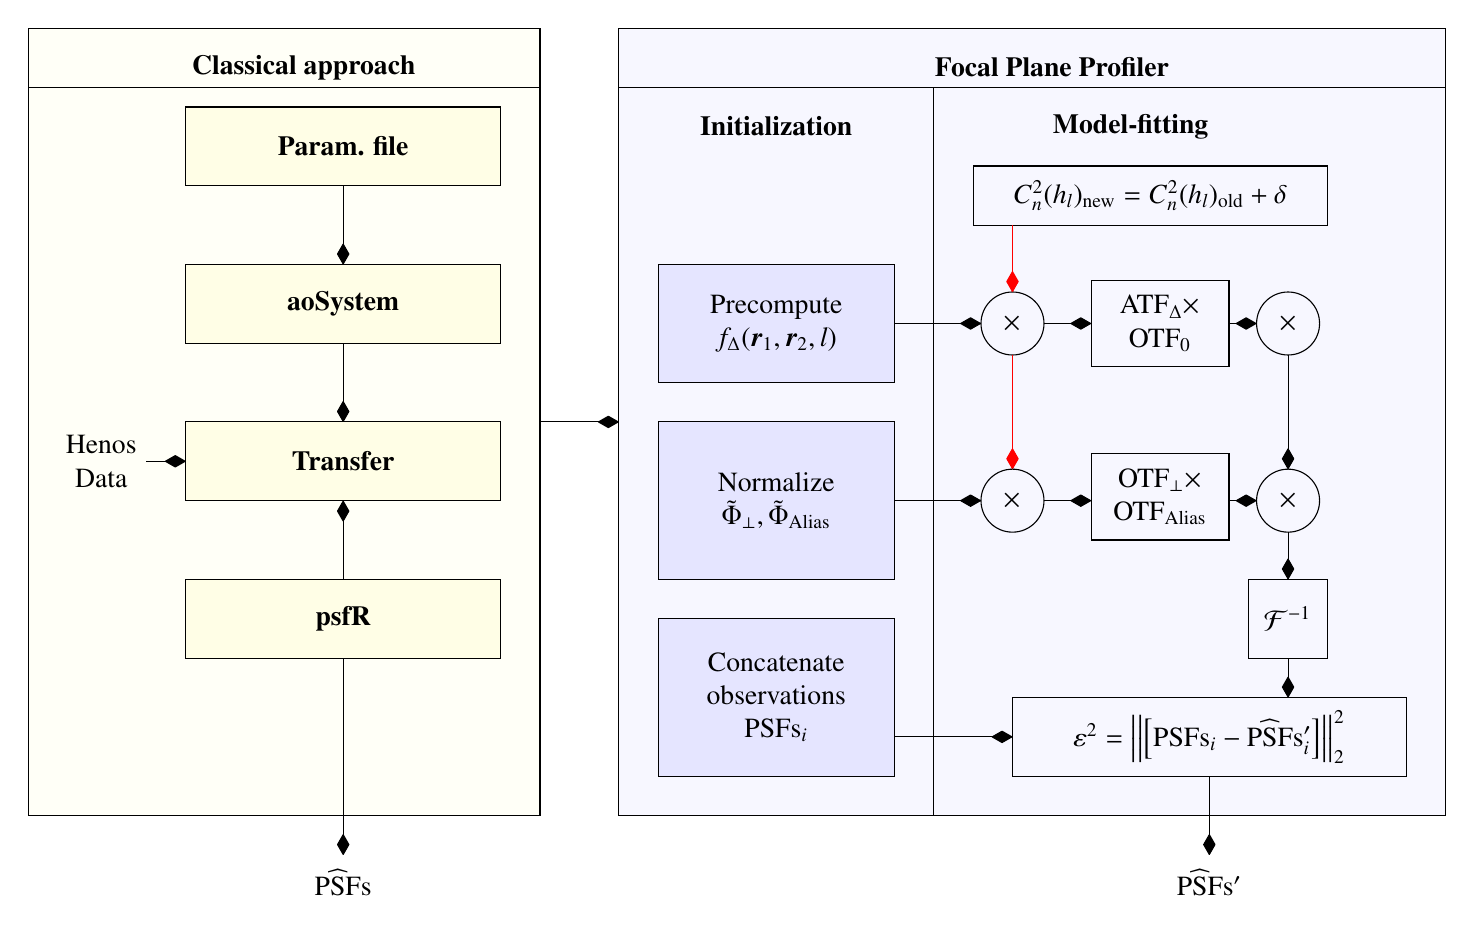
\begin{tikzpicture}[x=1cm,y=1cm,every text node part/.style={align=center}]	
	\draw[fill=yellow!3] (-2,0) rectangle(4.5,10);
	\draw(1.5,9.5) node{\textbf{Classical approach}};
	\draw(-2,9.25) -- (4.5,9.25);
	\draw[fill=yellow!10] (0,8) rectangle node{\textbf{Param. file}} (4,9);
	\draw[-diamond](2,8) -- (2,7);
	\draw[fill=yellow!10] (0,6) rectangle node{\textbf{aoSystem}} (4,7);
	\draw[-diamond](2,6) -- (2,5);
	\draw[fill=yellow!10] (0,4) rectangle node{\textbf{Transfer}} (4,5);
	\draw[-diamond] (-0.5,4.5)node[left]{Henos\\ Data} -- (0,4.5);
	\draw[-diamond](2,3) -- (2,4);
	\draw[fill=yellow!10] (0,2) rectangle node{\textbf{psfR}} (4,3);
	\draw[-diamond](2,2) -- (2,-.5);
	\draw(2,-.85) node{P$\widehat{\text{S}}$Fs};
	\draw[-diamond](4.5,5) -- (5.5,5);
	
	\draw[fill=blue!3] (5.5,0) rectangle(16,10);
	\draw(11,9.5) node{\textbf{Focal Plane Profiler}};
	\draw(5.5,9.25) -- (16,9.25);
	\draw(9.5,9.25) -- (9.5,0);
	\draw(7.5,8.75) node{\textbf{Initialization}};
		
	\draw[fill=blue!10] (6,5.5) rectangle node{Precompute\\ $f_\Delta(\rbun,\rbdeux,l)$} (9,7);
	\draw[fill=blue!10] (6,3) rectangle node{Normalize\\ $\tilde{\Phi}_\perp,\tilde{\Phi}_\text{Alias}$} (9,5);
	\draw[fill=blue!10] (6,.5) rectangle node{Concatenate\\ observations\\ PSFs$_i$} (9,2.5);
	\draw[-diamond](9,1) -- (10.5,1);
	\draw(12,8.75) node{\textbf{Model-fitting}};
	
	
	\draw(10.5,.5) rectangle node{$\varepsilon^2 = \norme{\cro{\text{PSFs}_i - \text{P}\widehat{\text{S}}\text{Fs}^\prime_i}}^2_2$} (15.5,1.5);
	\draw[-diamond](13,.5) -- (13,-.5);
	\draw(13,-.85) node{P$\widehat{\text{S}}$Fs$^\prime$};
	
	\draw(10,7.5) rectangle node{$\cnhl_\text{new} = \cnhl_\text{old} + \delta$} (14.5,8.25);
	\draw(10.5,6.25) circle(0.4) node{$\times$};
	\draw[-diamond] (9,6.25) -- (10.1,6.25);
	\draw[-diamond,color=red] (10.5,7.5) -- (10.5,6.65);
	\draw[-diamond] (10.9,6.25) -- (11.5,6.25);
	\draw (11.5, 5.7) rectangle node{ATF$_\Delta\times$\\OTF$_0$} (13.25,6.8);
	
	\draw[-diamond,color=red] (10.5,5.85) -- (10.5,4.4);
	\draw(10.5,4) circle(0.4) node{$\times$};
	\draw[-diamond] (9,4) -- (10.1,4);
	\draw[-diamond] (10.9,4) -- (11.5,4);
	\draw (11.5, 3.5) rectangle node{OTF$_\perp\times$\\OTF$_\text{Alias}$} (13.25,4.6);
	\draw(13.5,2) rectangle node{$\mathcal{F}^{-1}$}(14.5,3);
	\draw[-diamond](14,2) -- (14,1.5);
	\draw(14,4) circle(0.4) node{$\times$};
	\draw(14,6.25) circle(0.4) node{$\times$};
	\draw[-diamond](13.25,6.25) -- (13.6,6.25);
	\draw[-diamond](13.25,4) -- (13.6,4);
	\draw[-diamond](14,5.85) -- (14,4.4);
	\draw[-diamond](14,3.6) -- (14,3);
	\end{tikzpicture}
	\captionof{figure}{Focal plane profiler algorithm description using schema blocks.}
	\label{F:algo}
\end{center}


\section{Results on the NRC-HIA Henos testbed}

\subsection{System description}
All required parameters for PSF-reconstruction are introduced in~\cite{Rosensteiner2016}. Here is an exhaustive list of how the algorithm has been set up~:
\begin{table} [h!] 
	\centering
	\begin{tabular}{l|l}
		Source locations in x &11$\times$[-4.5,-4.5,4.5,4.5,-4.5]/2\\
		Source locations in y & 11$\times$[-4.5,4.5,-4.5,4.5]/2\\
		Guide star location   &11$\times$ [-4.5,-4/5]\\
		Sources wavelength    & 670 nm\\
		$r_0$                 &  0.584 @ 500 nm\\                             
		$L_0$                 & $\infty$\\		 
		fractional $r_0$      &  74.3\% ,17.4\%,8.2\% \\
		altitude layer        & (0.6, 5.2, 16.3) km\\
		source height         & 98.5 km \\
		Telescope diameter    & 8.13~m\\
		DM actuator pitch     & 0.813~m\\
		WFS sub-aperture spacing & 0.271~m
	\end{tabular}
	\caption{Summary of Henos set-up as inputs of the PSF reconstruction algorithm.}
	\label{T:par}
\end{table}

Note heights values are stretched by a factor eleven for reproducing the same anisoplanatism~(in my understanding) on NFIRAOS@TMT considering the given LGS separation.

\subsection{How to use the FocalPlaneProfiler class}

The FPP algorithm is embedded into the KASP architecture from the focalPlaneProfiler class. This later needs to be passed the psfR class~(see KASP notes\#03) for initializing the FPP algorithm and perform the model-fitting step. We describe below the piece of code allowing to use the FPP class. \\

When instantiating, the FPP class can be provided by flag, \emph{fitAlt} to identify altitude layers as well, as so as \emph{fitL0} to include the integrated outer scale~(fitL0=1) or outer scale profile~(fitL0=2) in the fitting process. If we do so, the computation time drastically increase from a minute up to 5 mn-ish because the pre-computation of the normalized covariance is no longer available since it depends on altitude and outer scale.

\begin{center}
	\framebox{
		\begin{minipage}{0.95\columnwidth}
			\textcolor{blue}{
				\begin{tabular}{ll}
					\multicolumn{2}{l}{\underline{\% Instantiating the aoSystem class}} \\
					sys     &= aoSystem('HenosSCAO','isSimu',false,'flagGaussian',true); \\
					sys	    &= instantiateHenosSystemClass(sys,pathData,object,pathCalib);\\
					\multicolumn{2}{l}{\underline{\% Instantiating the psfR class and run the reconstruction process}}\\
					psfr	&= psfR(sys,'flagGaussian',true);\\
					pr		&= psfr.getPSF('approach','old','method','slopes-based','samplingDomain','zonal');\\
					\multicolumn{2}{l}{\underline{\% Instantiating the focalPlaneProfiler class and run the profile estimation}} \\
					fpp		&= focalPlaneProfiler(psfr,'nLay',3,'fitL0h',0);\\
					fpp		&=fpp.getProfile();\\
					\multicolumn{2}{l}{\underline{\% Redo the psf reconstruction using retrieved $\cnh$ profile}}\\
					psfr	&= psfR(sys,'flagGaussian',true);\\
					pr		&= psfr.getPSF('approach','old','method','slopes-based','samplingDomain','zonal');\\
			\end{tabular}}
		\end{minipage}
	}
\end{center}

\subsection{FPP results}

\begin{table}
	\centering
	\begin{tabular}{|c|c|c|c|c|c|c|c|c|c|c|c|c|}
		\hline 
		& \multicolumn{3}{c|}{LGS 1} & \multicolumn{3}{c|}{LGS 2} &\multicolumn{3}{c|}{LGS 3} & \multicolumn{3}{c|}{LGS 4} \\
		\hline
		& Ref & PSF-R & FPP & Ref & PSF-R & FPP & Ref & PSF-R & FPP& Ref & PSF-R & FPP\\
		\hline
		SR [\%] 				& 43.7& 42.6 &42.6  &4.1   &3.8  & 3.0 & 6.0& 5.2 &  3.0 & 5.0&5.3 &4.2\\
		\hline
		FWHM [mas]				& 21.1& 22.6 & 22.6 & 116.6& 97	 &  112& 90 & 80  & 93  & 100& 77&91\\
		\hline
		EE 10$\lambda/D$[\%] & 78.8& 78.8 & 78.8 & 64.8 & 57	 &  55& 67 & 61  &   58.5& 64&59 &57\\
		\hline
		rms [counts]			& 0   & 251  & 250 & 0    & 3692&  3700& 0  & 1434&   1614& 0& 1597&1481\\
		\hline
	\end{tabular}
\end{table}

\begin{table}
		\centering
		\begin{tabular}{|c|c|c|c|c|}
			\hline
			& $\rz$ & $fr_0(1)$ & $fr_0(2)$ & $fr_0(3)$ \\
			\hline
			Ref & 82.97 cm & 74.3\%& 17.4\% &8.2\% \\
			\hline
			Fitted & 82.88 cm $\pm$ 2.07& 68.10\%$\pm$4.5 & 23.35\%$\pm$2.7&8.5\%$\pm$1.2 \\
			\hline
		\end{tabular}		
\end{table}

\begin{figure}
	\centering
	\includegraphics[scale=0.7]{/home/omartin/Projects/HENOS/results/psfrSCAOonaxis.pdf}
	\vspace{1cm}
	
	\includegraphics[scale=0.7]{/home/omartin/Projects/HENOS/results/psfrSCAOonaxis_2.pdf}
	\caption{On-axis psf reconstructed before~(\textbf{up}) and after~(\textbf{down}) $\cnh$ calibration using FPP. }
	\label{F:lgs1}
\end{figure}

\begin{figure}
	\centering
	\includegraphics[scale=0.7]{/home/omartin/Projects/HENOS/results/psfrSCAOoffaxis_lgs2.pdf}
	\vspace{1cm}
	
	\includegraphics[scale=0.7]{/home/omartin/Projects/HENOS/results/psfrSCAOoffaxis_lgs2_2.pdf}
	\caption{Off-axis LGS 2 psf reconstructed before~(\textbf{up}) and after~(\textbf{down}) $\cnh$ calibration using FPP. }
	\label{F:lgs2}
\end{figure}

\begin{figure}
	\centering
	\includegraphics[scale=0.7]{/home/omartin/Projects/HENOS/results/psfrSCAOoffaxis_lgs3.pdf}
	\vspace{1cm}
	
	\includegraphics[scale=0.7]{/home/omartin/Projects/HENOS/results/psfrSCAOoffaxis_lgs3_2.pdf}
	\caption{Off-axis LGS 3 psf reconstructed before~(\textbf{up}) and after~(\textbf{down}) $\cnh$ calibration using FPP. }
	\label{F:lgs3}
\end{figure}

\begin{figure}
	\centering
	\includegraphics[scale=0.7]{/home/omartin/Projects/HENOS/results/psfrSCAOoffaxis_lgs4.pdf}
	\vspace{1cm}
	
	\includegraphics[scale=0.7]{/home/omartin/Projects/HENOS/results/psfrSCAOoffaxis_lgs4_2.pdf}
	\caption{Off-axis LGS 4 psf reconstructed before~(\textbf{up}) and after~(\textbf{down}) $\cnh$ calibration using FPP. }
	\label{F:lgs4}
\end{figure}

\section{Conclusions}



\bibliographystyle{plain} 
\bibliography{/home/omartin/Documents/Bibliography/biblioLolo}

\end{document}
